\setstretch{1.5}
\chapter{Protocol}
\section{Introduction}
\subsection{Background}
Idiopathic Parkinson's disease (\acs{iPD})\acused{iPD} represents a chronic neurodegenerative disorder manifested by both motor and non-motor symptoms. The physical impairments in \ac{iPD} have a significant psychosocial impact and lead to considerable losses in patients'  \ac{QoL} and a high burden on (informal) caregivers. Several \ac{QoL} assessment tools have been developed so far, some of which are specific to \ac{iPD} \cite{stuhrenberg2022jpm}. However, none of the models take into account positive aspects of well-being or a subject's personal attitude (e.g., optimism) but also manifold aspects in someone's life such as lack of social support as possible stress factor or level of integration, to name a few.

This project will investigate the \ac{QoL} of patients with \ac{iPD} over time. To this end, a longitudinal assessment will be carried out using established and validated \ac{HRQOL} questionnaires. In addition, holistic observations will be collected using a questionnaire developed from the \textsc{CHAPO} model \citep{thieken2022jpd} -- an approach originally developed to assess quality of life in very old people\footnote{\url{https://ceres.uni-koeln.de/forschung/nrw80}}. This approach has been refined and will be adapted to aspects of \ac{iPD} patients for this cohort study. The aim of this project is therefore to record \ac{QoL} in a standardised way over a long period of time. These data will also be correlated with biomarkers obtained annually in the form of a cranial \ac{MRI} and blood, saliva, urine, hair and stool samples. We aim to identify biomedical markers with predictive value for changes in \ac{QoL}. In addition, the approach in this longitudinal study also aims to identify the support services needed to better meet the needs of \ac{iPD} patients' relatives. Carers' experience of stress, changes in sleep patterns and loss of \ac{QoL} over the observation period will be included in the analysis to identify a proxy for adequate support.

\subsection{Geographic context}
\AAcl{iPD} is one of the most common neurological disorders. Estimates put the incidence of the disease in Germany at \SI[round-precision = 1]{84.1}{} per \num[round-precision = 0, round-mode = places]{100000}{} people per year and assume a number of \num[round-precision = 0, round-mode = places]{400000}{} affected individuals \citep{nerius2017parkinson}. To understand the peculiarities of the \UKM{} regarding the care of \ac{iPD} patients, it is necessary to know the location of Marburg. About \SI[round-precision = 0, round-mode=places]{77000}{} people live in the city of Marburg, which is located in the countryside of central Germany. It is a university town and a district town in the federal state of Hesse (see figure \ref{fig1:hesseGermany}). Due to its location at about 80~km direct distance between the metropolitan areas of Frankfurt am Main and Kassel, the role of the \UKM{} must be understood as the predominant centre for medical care in the district. Approximately \num[round-precision = 0, round-mode = places]{1500}{} people with movement disorders are treated there every year. In order to ensure access to care for patients in the Marburg district, the department of neurology founded the \ac{PANAMA} in 2016. In this care network, various stakeholders work together to facilitate the integration of care services and improve outcomes for patients. At the same time, the university hospital is a tertiary centre that combines established treatment services for each stage of the disease with university medicine and offers a range of studies that can provide innovative forms of therapy. This allows offering modern, tailored treatments to people from outside the region.

\begin{wrapfigure}{r}{0.45\textwidth}
    \centering
    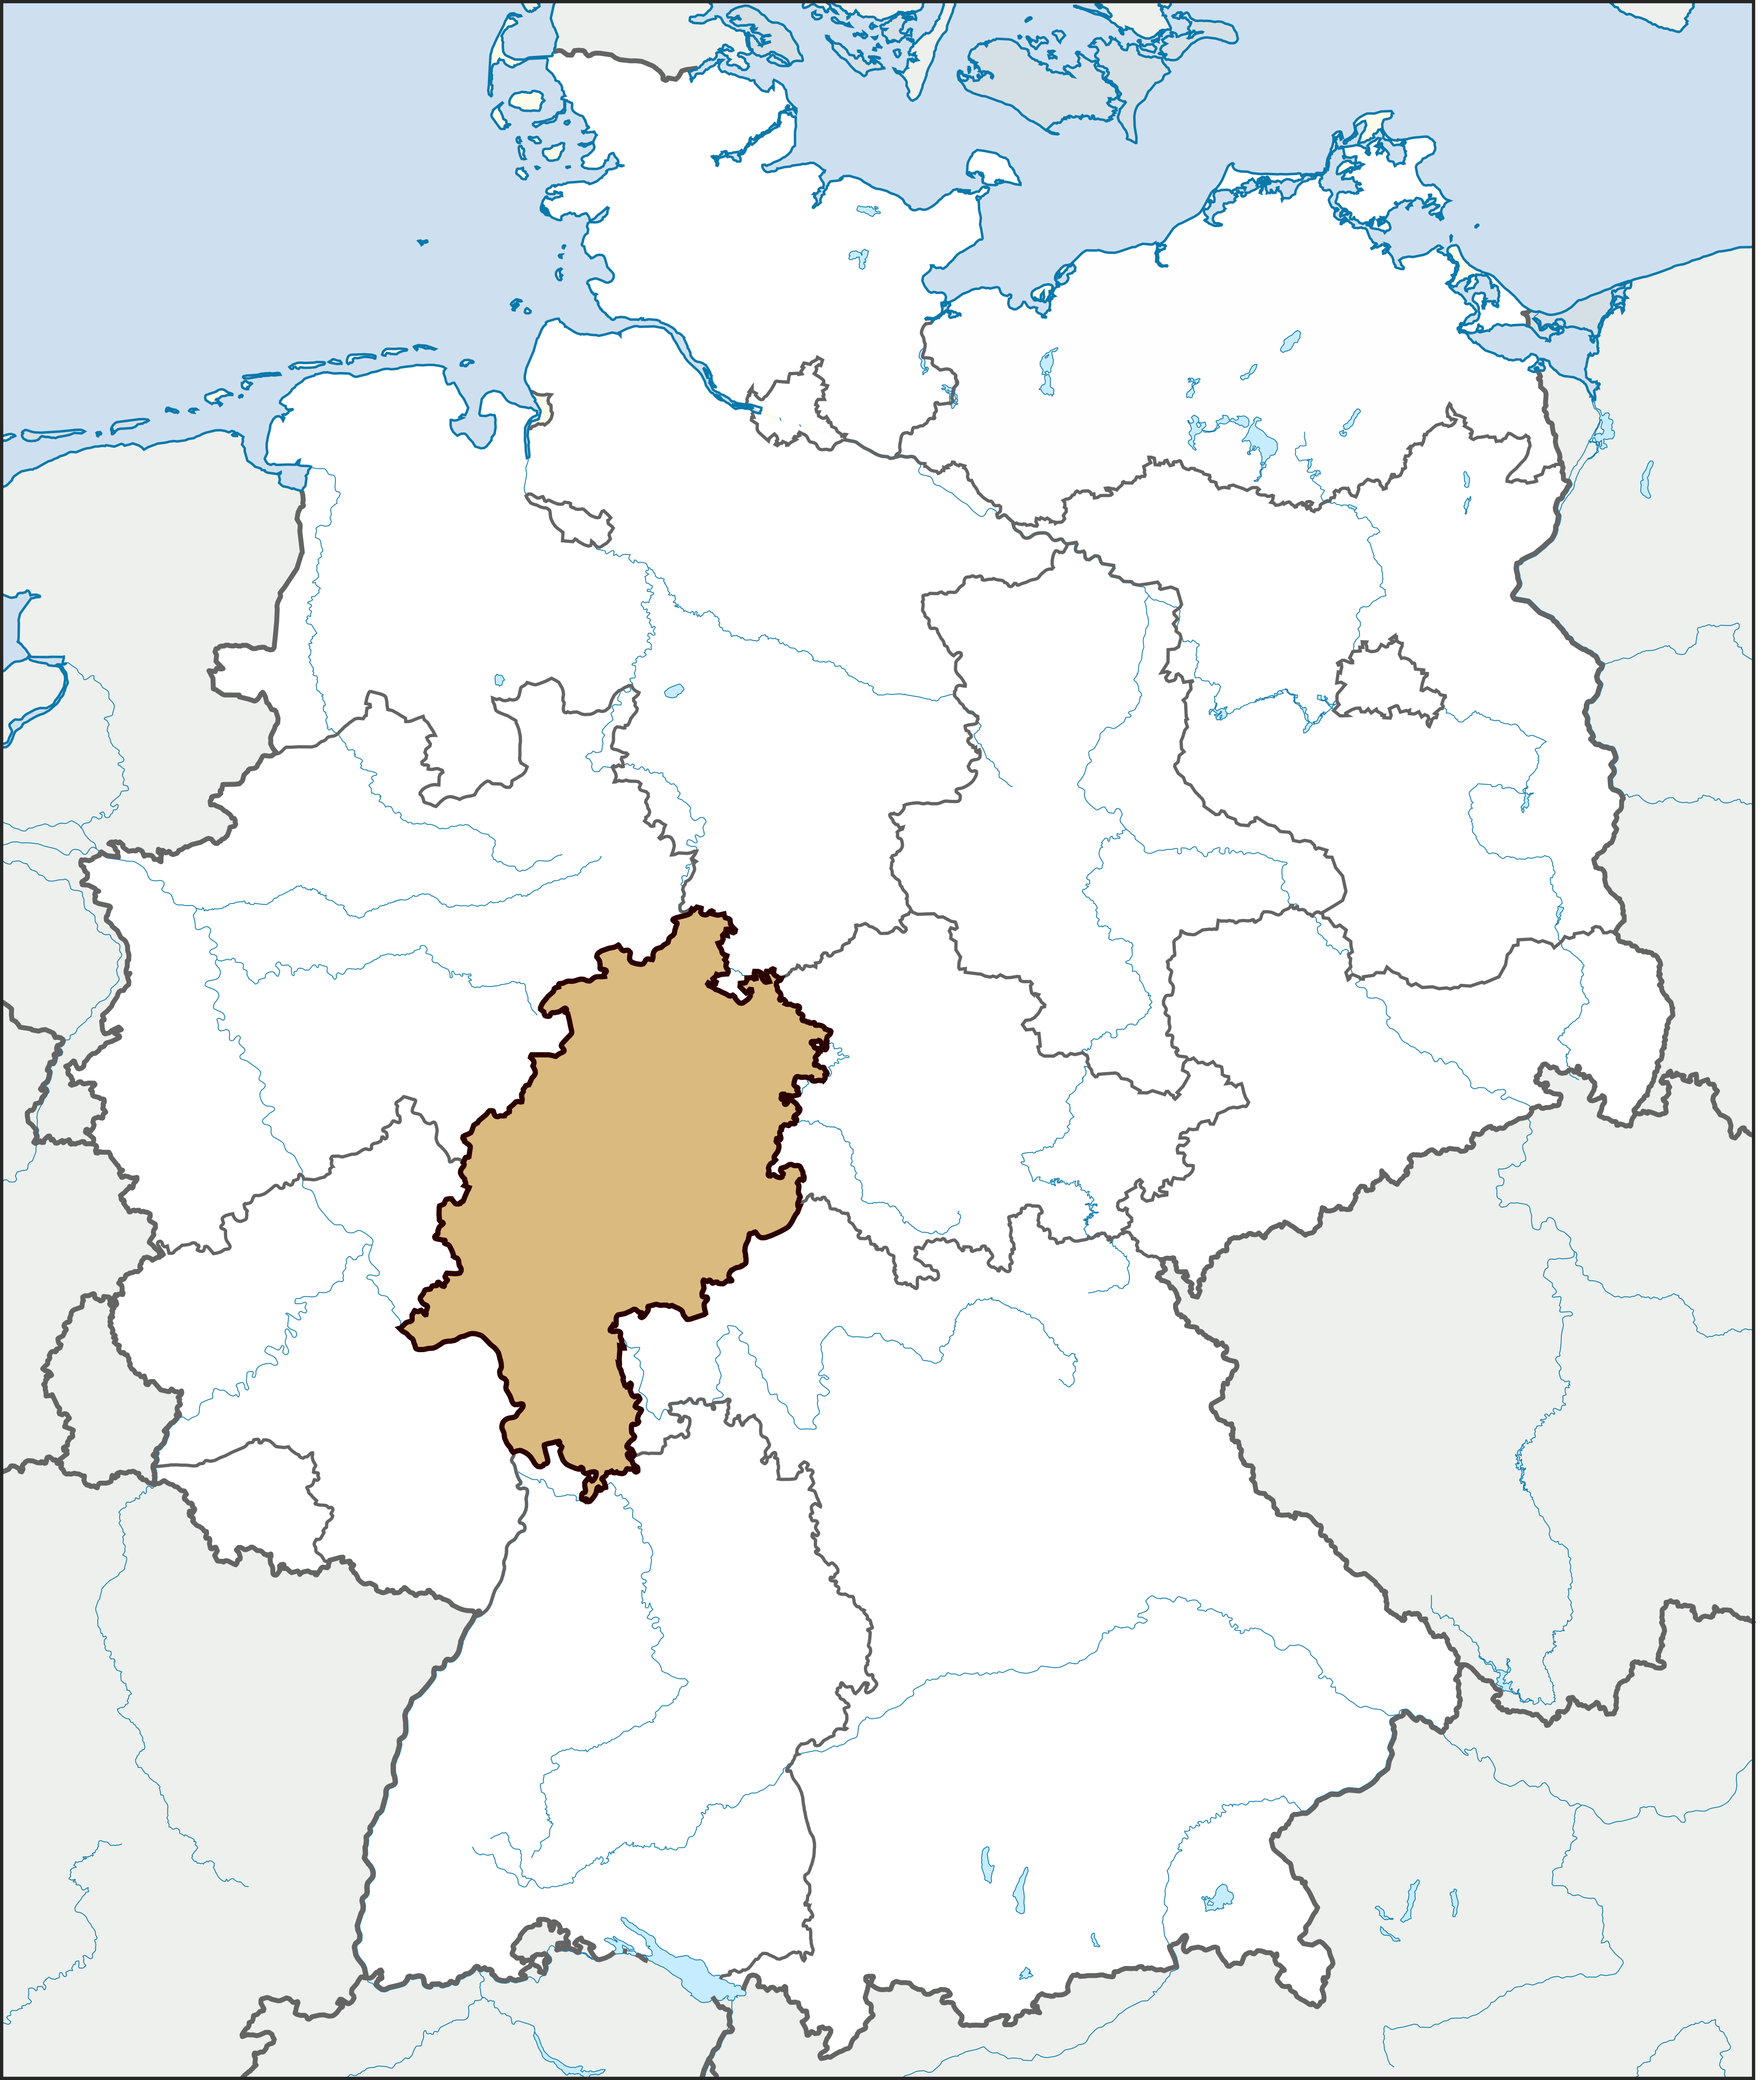
\includegraphics[width=0.45\textwidth]{Hesse_in_Germany.v1.0}
    \caption{Location of Hesse in the German Federal Republic}
    \label{fig1:hesseGermany}
\end{wrapfigure}

In order to represent the diversity of the population of \ac{iPD}-patients at \UKM{} and to ensure a balanced study cohort, as many of the treated patients as possible should be given the opportunity to participate in the \textsc{HessenKohorte}. Accordingly, the management of the study will adopt the recruitment strategies that have been successfully tested in previous clinical studies and to adapt them to the requirements of the long-term cohort study. To this end, on the one hand, patients are directly offered participation in the study during their appointments in the outpatient clinic of the hospital or during their inpatient stay in the neurology department. Secondly, members of \ac{PANAMA} will be made aware of the study with the aim of arousing the interest of potential participants. Finally, detailed information will be made available on the media website of \UKM{} to ensure sufficient information (\url{https://www.uni-marburg.de}).
\newpage

%%%%%%%%%%%%%%%%%%%%%%%%%%%%%%%%%%%%%%%%%%%%%%%%%%%%%%%%%%%%%%%%%%%%%%%
%%%% 										START OF SYNOPSIS												%%%%
%%%%%%%%%%%%%%%%%%%%%%%%%%%%%%%%%%%%%%%%%%%%%%%%%%%%%%%%%%%%%%%%%%%%%%%

\section{Protocol synopsis}
\inputtable{table_protocol_synopsis.tex}
\newpage

%%%%%%%%%%%%%%%%%%%%%%%%%%%%%%%%%%%%%%%%%%%%%%%%%%%%%%%%%%%%%%%%%%%%%%%
%%%% 										END OF SYNOPSIS													%%%%
%%%%%%%%%%%%%%%%%%%%%%%%%%%%%%%%%%%%%%%%%%%%%%%%%%%%%%%%%%%%%%%%%%%%%%%

\section{Study objectives and endpoints}
\subsection{Study objectives}
The primary aim of the \textsc{HessenKohorte} is to deepen the understanding of the development of \ac{QoL} in people with \ac{iPD} and to identify factors that have a beneficial or detrimental effect on it in a representative German cohort. In addition, the study aims to improve our understanding of the impact of the disease on caregivers and to find out which factors or forms of structural support make these carers more resilient to the stresses of caring for a person with \ac{iPD}.

\subsection{Primary study endpoint}
The primary endpoint of the \textsc{HessenKohorte} is the index patients' \ac{QoL}. A holistic measure of quality of life (\acl{HQ-PD}, \acsu{HQ-PD}) will be developed in a participatory approach with the \ac{iPD} participants which also measures others than disease-related aspects of quality of life and is based on earlier work with elderly patients (\acs{CHAPO-PD}).\ac{QoL} will will also be assessed using established questionnaires such as the \ac{PDQ39}\citep{jenkinson1997pdq39} or the assessment of the \ac{WHOQoL}\citep{group1998world}.

\subsection{Secondary study endpoints}
A large number of our measurements can be considered as secondary endpoints. Due to the many different  measurements taken and the long data acquisition time of the study a large number of analyses will be possible. A non-exhaustive list of possible secondary endpoints shall be named here:
\begin{itemize}[noitemsep,topsep=0pt]
  \item{Changes in motor symptoms of the index patient over the course of the study}
  \item{Development of non-motor symptoms over time}
  \item{Changes of the structural imaging over time and their relationship
        to other symptoms} 
\end{itemize}
Notwithstanding the unique characteristics of a study of the \ac{QoL} of people with \ac{iPD}, standard examinations of \ac{iPD} patients should also be carried out as far as the secondary endpoints are concerned. At this point, motor and non-motor symptoms should be mentioned as the most commonly encountered symptoms. The former are the hallmark of the disease, while the latter are increasingly recognised as responsible for huge losses in \ac{QoL} \citep{klietz2020qol}. The extent of motor symptoms is operationalised by Part III of the \ac{MDS-UPDRS}\cite{goetz2007updrs}. Non-motor symptoms will be measured using the \ac{NMSQ}, a measure capable of capturing a wide range of different aspects of this symptom domain. An overview of the scheduled time points for all questionnaires can be found in Table \ref{tab:questionnaireSchedule}.

\section{Study design}
The \textsc{HessenKohorte} is a longitudinal, observational, natural history study to assess the \ac{QoL} progression of study participants with \ac{iPD}. The planned cohort size of \num[round-precision = 0, round-mode = places]{1000}{} will be comprehensively assessed over a maximum of twenty years. All subjects and their relatives will undergo clinical examinations and patients will be regularly assessed for motor, non-motor, cognitive and neuropsychiatric symptoms as well as \ac{QoL}. Imaging studies will also be undertaken and patients will be asked to provide biospecimens including blood, urine, saliva, hair and faeces. All carers will be asked to complete questionnaires and provide digital data as part of the \textsc{HessenKohorte}.

\subsection{Scale and duration}
The study will accompany up to \num[round-precision = 0, round-mode = places]{1000}{} patients over at most 20 years to enable a profound insight into the life course of patients' and relatives' \ac{QoL}.

\subsection{Justification for study design}
The \textsc{HessenKohorte} is a single-centre, longitudinal, observational follow-up study of the holistic \ac{QoL} of patients with \ac{iPD}. This unique primary endpoint will be assessed using a newly developed questionnaire (\ac{HQ-PD}), the main feature of which is a holistic assessment that looks not only at disease-related limitations but also at the existing resources and social environment of those affected \cite{thieken2022jpd}. Accordingly, the involvement of relatives is fundamental to understanding the impact of the disease on the patient's entire environment. The comparatively large number of subjects should provide a good insight into the lives of \ac{iPD} patients with their diverse phenotypes, but also offer opportunities for diverse investigations through the additional collection of biospecimens.

\subsection{Hypotheses}
\label{sec:hypoTheses}
The primary endpoint of the study is the development of \ac{iPD}-patients' \ac{QoL} over the course of up to 20 years. The \textsc{HessenKohorte} thereby addresses the following main scientific hypothesis:
\begin{itemize}
  \item Exploratory analysis of the development of \acl{QoL} over the course of the disease.
\end{itemize}
The design of the study is based on the currently accepted assumption that the \ac{QoL} of people with PD is significantly correlated with the severity of symptoms. It can also be assumed that the \ac{QoL} of people with PD is strongly related to that of their relatives. The present study design is intended to contribute to the longitudinal assessment of \ac{QoL}, but in particular to allow exploratory studies during or at the end of the data collection, which could provide information on whether certain factors found in the behavioural data, imaging or biospecimens might have a predictive value for changes, but especially for reduced QoL.

\subsection{Planned analyses}
Our main method for assessing the hypotheses are \ac{ANOVA}, linear regression and correlation analyses. In particular we will analyse the correlation between the \ac{QoL} of the index patient and of her relatives and caregivers. In order to extend this analysis we will assess different influencing factors as, e.g., age, gender and symptom burden (motor and non-motor). Furthermore in an attempt to elucidate the causal form of the interdependence we will analyse how \ac{QoL} of patients/caregivers at earlier timepoints relates to \ac{QoL} of caregivers/patients at a later point in time.

With regard to our hypothesis concerning the prediction of disease progress, we will primarily rely on linear and regression methods. We will try to offer models predicting disease symptoms at the end of the study compared to the status at earlier timepoints. While we first will look at a linear relationship we will also consider more complicated models when they are necessary to model disease progress convincingly. Also in this analysis mediating or moderating variables especially from sociodemographic data may play a role and will accordingly be considered.

\begin{figure}[h]
\label{fig2:scheme}
\centering
\includegraphics[width=1\textwidth]{Schema_HessenKohorte.v2.0}
\caption{Schematic overview of the planned data collection. Subjects will be enrolled subsequently and will receive regular follow-ups. In addition to clinical data in form of different questionnaires, which will be assessed semiannually, biomarkers including cranial \ac{MRI}, blood, saliva, urine, hair and stool samples will be collected annually.}
\end{figure}


\section{Subject selection}
\label{sec:study_selection}
\subsection{Study population and Eligibility}
\label{sec:study_population}
Study candidates will be drawn from the patients treated in the neurology department of the \UKM{}, as either in- or outpatients. Moreover, all patients in the federal state of Hesse suffering from \ac{iPD} may submit a request for participation in the study. The inclusion and exclusion criteria (cf. Section \ref{sec:inclusion_criteriaIPS}) are checked by one of the study physicians, who are responsible for the final decision. Advertising for the study can be found in the form of a flyer, which is available in the Department of Neurology, but also in the form of an internet homepage, where the project will be presented to the public and we will also promote study participation over the \ac{PANAMA} network (\url{https://www.parkinson-marburg.com}).

\subsection{Inclusion and exclusion criteria for \ac{iPD}-patients}
\label{sec:inclusion_criteriaIPS}
Subjects who meet all the following inclusion criteria may be given consideration for inclusion in this cohort study, provided no exclusion criteria are met (for both, cf. Table \ref{tab:inclusionexclusionCriteriaPatients}).

\inputtable{table_inclusion_and_exclusion_criteria_patients.tex}

\subsection{Inclusion criteria for \ac{iPD}-patients' relatives}
\label{sec:inclusion_criteriaREL}
Only if a patient is included, the relatives may be asked for participation in the study. Subjects who agree to take part in the \textsc{HessenKohorte} must meet all of the following inclusion and exclusion criteria (cf. Table  \ref{tab:inclusionexclusionCriteriaRelatives}).

\inputtable{table_inclusion_and_exclusion_criteria_relatives.tex}

\section{Subject accountability}
\subsection{Point of enrollment}
Subject will be considered to be enrolled at the time of the study-specific \ac{ICF} execution. No study-related procedures or assessments can take place until the \ac{ICF} is signed.

\subsection{Withdrawal}
All enrolled subjects (including those who have dropped out) must be recorded and documented. In case participants drop out of the study, an end-of-study form (cf. Appendix \ref{sec:eos_form}) must be filled out and the reasons for dropping out are assessed. 

Reasons for withdrawal include but are not limited to:
\begin{itemize}
  \item subject or relative choice to withdraw consent
  \item lost to follow-up
  \item pregnancy\footnote{\label{note1} only MR-imaging will be discontinued during pregnancy or from the moment of an implantation onwards.}
  \item implantation of electrical devices or metal parts in or on the body\footref{note1}
\end{itemize}

Subjects may withdraw at any time, with or without reason, and without prejudice to further treatment. The applicable \ac{CRF} up to the point of subject withdrawal and an \hyperref[sec:eos_form]{end-of-study form} must be completed. A minimum of three documented attempts to contact any subject considered lost to follow-up should be made prior to completion of the end-of-study form. No further study data should be collected after the point at which a subject is withdrawn from the study or withdraws consent, for whatever reason. Data collected up to the time of subject withdrawal may be used.

\subsection{Lost to follow-up}
Patients who do not react to the invitation to fill out the questionnaires will be contacted in total three times per mail or email:
\begin{itemize}
\item 30 days before the planned visit
\item at the date of the visit and
\item 30 days thereafter
\end{itemize}
If there is no response to the third contact attempt, patients are contacted by telephone to find out if there is a problem. Patients who cannot be contacted will receive the same number of mails/calls after one and two years. If there is no response for three years, an end of study form (cf. Appendix \ref{sec:eos_form}) will be completed and the subject will be excluded. Vacancies due to excluded subjects may be filled 5 and 10 years after the start of the study.

\subsection{Subject status and classification}
A subject will be considered enrolled in this study at the time of the study-specific \ac{ICF} execution.

\subsection{Enrolment control}
The overall enrollment in the study will be capped at \num[round-precision = 0, round-mode = places]{1000} patient participants, i.e., potentially \num[round-precision = 0, round-mode = places]{2000} patients with their respective caregivers.

\subsection{End-of-study definition}
The study is considered complete when 20 years from the first enrolment are over in the year 2043.

\section{Study methods}
\subsection{Data collection}
The data collection schedules are shown in Tables \ref{tab:DataCollectionPatients} and \ref{tab:DataCollectionRelatives}.
\inputtable{table_data_collection_schedule_patients.tex}
\inputtable{table_data_collection_schedule_relatives.tex}
%Urs: Bitte angleichen an das Protokoll zur Veröffentlichung
%David: %dort haben wir ja aktuell eine andere Tabelle: Frageboegen und andere
%Datenquellen in einer Tabelle. Willst Du das hier auch so? Ich finde
%es eigentlich so wie es hier ist besser.

\subsection{Candidate screening}
\label{subsec:screening}
Subjects will be screened for participation in the study based on study inclusion and exclusion criteria as listed in Section \ref{sec:study_selection}. Subjects who have provided informed consent and who have been determined to not meet all eligibility requirements will not be considered.

\subsection{Informed consent}
Written informed consent must be obtained from potential study candidates and enrollment is only valid after subjects sign and date the \ac{ICF}. The informed consent forms of this study can be found in the appendices \label{sec:icf_patient} and \label{sec:icf_relative} respectively.

\begin{itemize}[noitemsep, topsep=0pt]
\item Subjects will be asked to sign the \ac{ICF} before study-specific tests or procedures are performed.
\item The idea of the study must be explained, and subjects must be given the time and opportunity to ask questions and have those questions answered to their satisfaction.
\item The \ac{ICF} is study specific and has been approved by the ethics commitee.
\item Written informed consent must be recorded appropriately by means of the subject’s dated signature.
\end{itemize}

\subsection{Questionnaires}
\label{subsec:questionnaires}
\subsubsection{\acl{HQ-PD}}
\label{questionnaires:holy}
The backbone of the study will be the investigation of \ac{QoL}. Recent debates suggest that established measurement tools do not capture \ac{QoL} with a holistic view but focus on the health-related experience of \ac{QoL} \cite{stuhrenberg2022jpm,Karimi2016}. Furthermore, it is unclear to date what determinants influence \ac{QoL} beyond mere disease in \ac{iPD}. It is also unclear how \ac{QoL} develops over the course of the disease. The HessenKohorte offers a unique opportunity to capture changes in \ac{QoL} in a large study population and develop a comprehensive understanding of this important concept. The study therefore pursues two goals: (i) the development and validation of a holistic measurement instrument for the assessment of \ac{QoL} and (ii) the longitudinal observation of \ac{HRQOL} using established measurement instruments (cf. Table 1). 
To fulfil the first goal, an instrument, the \ac{HQ-PD}, will be developed in the first year of the cohort in an evidence-based, patient-oriented and participatory manner, which will be validated alongside the cohort from the second year onwards.  This means that in addition to a systematic review of existing studies, \ac{iPD} patients will be interviewed about their personal experience of \ac{QoL} and actively involved in the development process of the instrument according to the INVOLVE-guideline\footnote{\url{https://www.invo.org.uk/wp-content/uploads/2019/04/Copro_Guidance_Feb19.pdf}}. In this process, the study team is guided by the work from the NRW80+ study in which the experience of \ac{QoL} of elderly people was investigated for the first time in Germany \cite{wagner2017}.

\subsubsection{\acf{MDS-UPDRS}}
\label{questionnaires:updrs}
The \ac{MDS-UPDRS} \cite{goetz2007updrs} evaluates various aspects of \ac{iPD}-patients, including non-motor and motor symptoms. It consists of four parts:
\begin{itemize}
\item Part I: Experiences of daily living (non-motor symptoms), including 13 items.
\begin{itemize}
\item A: Behavioural problems of the patient, as evaluated by the examiner.
\item B: Part on non-motor symptoms completed by the patient, with the assistance of a caregiver if necessary, but independent of the investigator.
\end{itemize}
\item Part II: Experiences of daily living (motor aspects) with 13 items. This part is also a self-report questionnaire to be completed by the patient, with the assistance of a caregiver if necessary, but independent of the investigator.
\item Part III: Motor examination with 18 items. All instructions are read to the patient by the examiner or demonstrated directly, so that this part is completed by the examiner.
\item Part IV: Motor Complications with 6 items. This part contains instructions for the examiner and also instructions to be read to the patient. It combines patient-related information with clinical observations and assessments by the examiner.
\end{itemize}

\subsubsection{\acf{MoCa}}
\label{questionnaires:MoCa}
The \acl{MoCa} evaluates the performance in different cognitive domains. The questions test cognitive abilities such as memory, language production, contextual thinking, attention and concentration, behaviour, arithmetic, temporal and spatial orientation, and the ability to recognize complex shapes and patterns. Scores result from the correct completion of the tasks, whereby the cognitive performance in the individual domains but also as an overall score can be quantified. The \ac{MoCa} was developed in 2005 \cite{nasreddine2005moca} and has been used in clinical practice since then. The test must be administered by a trained examiner and an assessment sheet, a pen and stopwatch are needed. The duration is about \num[round-precision = 0, round-mode=places]{10} \SI{}{\minute}.

\QScores{}
\begin{itemize}\itemsep2pt
\item 30--26: normal
\item 25--21: \ac{MCI}
\item $<$ 21: dementia
\end{itemize}

\QPsychometrics{}
\inputtable{table_psychometrics_moca.tex}

\subsubsection{\acf{NMSQ}}
\label{questionnaires:NMSQ}
The \ac{NMSQ} is a 30-item rater-based scale designed to assess a broad spectrum of non-motor symptoms in patients with \ac{iPD}.
The scale is scored by clinicians and consists of 30 items assessing nine domains of non-motor symptoms, including (1) cardiovascular, (2) sleep/fatigue, (3) mood/apathy, (4) cognition/hallucinations, (5) attention/memory, (6) gastrointestinal, (7) urinary, (8) sexual function, and (9) miscellaneous. The miscellaneous category includes questions about pain, smell/taste, weight change and excessive sweating. The total score ranges from 0, indicating no impairment, to 360, indicating maximum impairment, with symptoms assessed over the past four weeks. 

\subsubsection{\acf{BDI}}
\label{questionnaires:BDI}

The \acl{BDI} measures the severity of depressive symptoms. It consists of 21 items  measuring symptoms on a scale from 0--3. The questionnaire was first introduced in 1991 \cite{beck1987bdi1} and revised to the current version in 1996 \cite{beck1996bdi2}. The self-administered test takes 5-10 minutes to complete but does not require any special training. Answers are added for the total score, so that results range in a scale of 0--63 points. Higher scores thereby correspond to more severe symptoms. Since its development, the \ac{BDI} has been used to quantify depressive symptoms in non-specific populations, but particularly in patients with stroke, spinal cord injury and \ac{iPD}. 

\QScores{}
\begin{itemize}\itemsep2pt
\item 0--12: no depressive symptoms or clinically inapparent
\item 13--19: mild depressive syndrome
\item 20--28: moderate depressive syndrome
\item $>$ 29 severe depressive syndrome
\end{itemize}

\QPsychometrics{}
\inputtable{table_psychometrics_bdi.tex}

%\subsubsection{\acl{CBI} (\acs{CBI})}
\subsubsection{\acf{CBI}}
\label{questionnaires:CBI}
The \acl{CBI} assesses the presence or severity of symptoms indicative of burnout. In the short version used here, the questionnaire consists of 19 items that scale levels of physical and psychological exhaustion in relation to personal, work and client burnout. The CBI was introduced in 2005 by Kristensen et al. \cite{kristensen2005cbi} and is self-administered without special training. It takes about 5-10 minutes to complete. The scale ranges from 1 (``never/very seldom'' or ``to a very low degree'') to 5 (``very often'' or ``to a very high degree''), resulting in a total score of 19--95 by adding the individual scores or individual scales for personal burnout (6--30), work-related burnout (7---36) and client-related burnout (6--30). A higher score indicates higher levels of stress and an increased likelihood of burnout.

\QPsychometrics{}
\inputtable{table_psychometrics_cbi.tex}

\subsubsection{\acf{CISS}}
\label{questionnaires:CISS}
The \acl{CISS} assesses habitual coping with stress in the context of task-oriented coping, emotion-oriented coping and avoidance-oriented coping with a total of 24 and 48 questions respectively. The CISS was originally introduced in 1990 \cite{endler1990ciss} and revised in 2020 for a shortened German version \cite{kalin2020ciss}. The questionnaire is self-administered without special training and takes 10 to 15 minutes to complete. Three distinct domains of coping (task-, emotion- and avoidance-oriented coping) can be identified using a normogram and according to the respective questions. The test is not validated for sequential administration and is therefore administered once every 5 years.

\QPsychometrics{}
\inputtable{table_psychometrics_ciss.tex}

\subsubsection{\acf{MFI-20}}
\label{questionnaires:MFI20}
The \acl{MFI-20} measures five dimensions of fatigue with 20 questions: general fatigue, physical fatigue, reduced activity, reduced motivation and mental fatigue. The \acs{MFI-20} was introduced in 1995 \cite{smets1995mfi20}. It is a self-administered test that requires no special training and is reported to take 5 - 10 minutes to complete. It includes response options to various fatigue-related statements ranging from ``Yes, this is true'' to ``No, this is not true'', scaled from 1 -- 5 per question, with 4 -- 20 points for each dimension. A high total score on the different dimensions corresponds to a higher level of fatigue in the corresponding dimension.

\QPsychometrics{}
\inputtable{table_psychometrics_mfi20.tex}

\subsubsection{\acf{PDCB}}
\label{questionnaires:PDCB}
The Parkinson's Disease Caregiver Burden Questionnaire (\acs{PDCB}) measures level of burden experienced in caring for a person with \ac{iPD}. It consists of 20 questions in 8 domains that indicate the occurrence of various emotional, health and social consequences of caring for persons with \ac{PD}, using a 0 to 4 point scale by disagreeing (``I disagree'') and gradually increasing agreement (``I strongly agree'') with statements about one's burden. The (\acs{PDCB}) was first introduced in 2013 \cite{zhong2013pdcb}, and revised in 2019 with a German translation \cite{klietz2019pdcb}. It takes 5 - 10 minutes to complete and is a self-administered test that requires no special training. The total score of the questionnaire is obtained by adding the individual scores between 0 -- 4 of all 20 questions. A higher score corresponds to a greater burden of caring for a person with \ac{PD}.

\QPsychometrics{}
\inputtable{table_psychometrics_pdcb.tex}

\subsubsection{\acf{PHQ}}
\label{questionnaires:PHQ}
The \acs{PHQ} is an instrument for the diagnosis of mental disorders that assesses various somatic, psychological and stress-related complaints on the basis of 16 domains. The \acs{PHQ}, which is based on DSM-IV criteria, was introduced for psychodiagnosis in the USA in 1999 \cite{spitzer1999phq} and validated in 2002 as the ``Health Questionnaire for Patients (PHQ-D)'' in a German version \cite{lowe2002phq}. It takes about 15 minutes to complete and is self-administered. Nine of the items (2a--2i) measure ``depressiveness''. The response categories are as follows: 0 (``not at all''), 1 (``on some days''), 2 (``on more than half of the days'') and 3 (``almost every day''), giving a total score of 0--27. Scores below 5 points indicate no depressive symptoms, 5--10 points indicate mild depressive symptoms and all scores above 10 points indicate major depression (moderate, marked or severe). A further 15 items (1a--1m, 2c, 2d) measure somatic symptoms, resulting in a scale total for the ``somatic symptoms'`'. Of these, 13 items are scored as: 0 (``not impaired''), 1 (``slightly impaired'') or 2 (``severely impaired''). In addition, two items from the depression section are scored as: 0 (``not at all''), 1 (``on some days''), 2 (``on more than half of the days'') and 3 (``almost every day''). The total score ranges from 0--30 points, with higher scores corresponding to greater somatoform distress. 
A severity score for the stress domain can be obtained by summing items 12a--12j to obtain a scale total. The numerical rating of the individual items is 0 (``not affected'), 1 (``slightly affected') or 2 (``severely affected'). Accordingly, the total stress score varies between 0 and 20, with higher scores corresponding to greater stress.

\QPsychometrics{}
\inputtable{table_psychometrics_phq.tex}

\subsubsection{\acf{PSS}}
\label{questionnaires:PSS}
The \ac{PSS} is a self-report measure of the extent to which the respondent has found situations in his/her life stressful in the past month and includes both a helplessness scale and a self-efficacy scale. It consists of 10 questions measuring the frequency of feeling stressed in the past month on a scale from ``never'' to ``almost always'', corresponding to a point scale between 1 and 5. The \ac{PSS} was first introduced in 1983 \cite{cohen1983pss} and revised in 2010 \cite{schneider2020pss}. It takes about 5 minutes to complete and requires no special training. The helplessness scale is the sum of items 1, 2, 3, 6, 9, 10; the self-efficacy scale is the sum of items 4, 5, 7, 8. To calculate the total score, items 4, 5, 7 and 8 of the self-efficacy scale must be inverted. The total score is the sum of the helplessness scale items and the sum of the inverted self-efficacy scale items. Higher scores indicate greater distress.

\QPsychometrics{}
\inputtable{table_psychometrics_pss.tex}

\subsubsection{\acf{WHOQoL}}
\label{questionnaires:WHOQoL}

The \ac{WHOQoL} questionnaire measures subjective quality of life in adulthood and consists of a total of 26 items divided into 4 domains: physical quality of life, psychological quality of life, social relationships and environment. In addition, global quality of life and general health are measured by 2 additional items. The questionnaire was introduced in 1996 \cite{world1996whoqol} on behalf of the \ac{WHO} and has been used in German translation since 2002 \cite{gunzelmann2002whoqol}. The time required to complete the questionnaire is given as 10 - 15 minutes. Based on the response options, the domains are scored on a point scale (1-5) as follows, with higher scores corresponding to better quality of life:

\QScores{}
\begin{itemize}\itemsep2pt
\item Physical health: 7 -- 35 points
\item Psychological Health 6 -- 30 points
\item Social relationships 3 -- 15 points 
\item Environment 8 – 40 points
\end{itemize}

\QPsychometrics{}
\inputtable{table_psychometrics_whoqol.tex}

\subsection{Biosamples}
\label{subsec:biosamples}
The collected blood, urine, saliva and faeces samples are immediately processed at the \ac{CBBMR}. Processing is carried out by an experienced team to the highest international standards. Water is offered at the beginning of each visit to enable the participants to provide saliva and urine more easily.

\subsubsection{Blood}
\label{biosamples:blood}
Blood samples will be collected for blood count and genetic analyses:
\begin{itemize}
\item \acs{EDTA} (35ml) for \acs{DNA} extraction, plasma preparation and blood count
\item PAXgene\textsuperscript{TM} (Becton-Dickinson, Heidelberg, Germany) system
      for transcriptome information
\item \acs{CPT} Vacutainer (8ml, Becton-Dickinson, Heidelberg, Germany)
      for obtaining \acsp{PBMC}
\end{itemize}
A maximum of \SI[round-precision = 0, round-mode = places]{55}{\milli\litre} will be collected at each visit and it is strongly recommended that research blood samples are collected in a fasted state (i.e. at least 8 hours since last meal/food intake) to ensure sample quality for future analysis. If fasting is not possible, participants should be advised to follow a low fat diet. All research samples will be sent to a central biorepository for indefinite storage for research purposes. Samples will be made available to researchers for analysis in relation to \ac{iPD} and other diseases. \\

\noindent \underline{Required materials}:
\begin{itemize}
  \item 1 $\times$ 4.6ml \acs{EDTA} (blood count)
  \item 2 $\times$ 9ml \acs{EDTA} Sarstedt K2 ref. 02.1333.001 
  \item 1 $\times$ 8ml \acs{CPT} (Sodium Citrate) ref. BD 362782
  \item 1 $\times$ PAXgene\textsuperscript{TM} ref. BD 762165
  \item 1 $\times$ 15ml Falcon tube conical 
  \item 10 $\times$ 1 ml Fluid X tubes 96 ref. Brooks 68-1001-11 
\end{itemize}


\subsubsection{Urine}
\label{biosamples:urine}
Midstream urine (approximately 40 ml) will be collected during the visit. After collection urine is centrifuged and supernatant will be aliquoted and stored at -80°C for later analysis. Pellets will be re-suspended in DNA/RNA Zymo research shield (Biozol, München, Germany) for  nucleid acid analysis.

\noindent \underline{Required materials}:
\begin{itemize}
  \item 1 $\times$ 40ml urine sample
\end{itemize}

\subsubsection{Saliva}
\label{biosamples:saliva}
Two saliva collections will be performed with different objectives. One is used for metabolomic analysis in \ac{iPD} patients and the second is for DNA extraction. Saliva withdrawals are self-administered by the patient after proper instruction.

For metabolomics, saliva is collected using a Salivette\regd{} (Sarstedt, Nümbrecht, Germany). The Salivette tubes including the saliva enriched gum are centrifuged before the gum is discarded.  The homogenised samples are then aliquoted at \SI[round-precision = 0, round-mode = places]{150}{\micro\litre} and stored at \SI[round-precision = 0, round-mode = places]{-80}{\degreeCelsius}.

DNA extraction from saliva samples is performed using the SalivaGene Collector system. Samples are stored at \SI[round-precision = 0, round-mode = places]{-80}{\degreeCelsius} for up to \num[round-precision = 0, round-mode = places]{12} months and then processed in the \ac{CBBMR} applying preparation with the SalivaGene DNA Kit (Invitek, Berlin, Germany).

\noindent \underline{Required materials}:
\begin{itemize}
\item Invitek SalivaGene Collection Module II (Artikelnummer: 10 352 122 00)
\item Sarstedt Salivette (Artikelnummer: 51.1534.500)
\end{itemize}

\subsubsection{Hair}
\label{biosamples:hair}
Metabolomics is a useful tool for identifying biomarkers of disease and uncovering pathogenic mechanisms \cite{Chen2021}. However, most metabolomic studies use biological fluids such as blood and urine as biospecimens, which can be dramatically affected by daily activities and dietary variations, resulting in measurement variability. In contrast, hair can serve as a robust source of stable longitudinal metabolite information. Human hair grows at a rate of approximately \num{1} \SI{}{\centi\metre} per month, with both endogenous compounds and environmental factors being incorporated into the hair during growth. Therefore, we plan to analyse hair metabolomics over time during the course of the study. For this purpose, an in-house questionnaire on hair characteristics and products used has been developed and will be administered to all patients. A specific protocol has been developed for hair collection, including standardised location of hair to be collected, technique and processing. 

Hair samples will be taken from the posterior vertex using a standardised procedure. Along with a questionnaire asking about the use of specific products, 2-3 strands of hair are cut as close to the skin as possible. The collected hairs are wrapped in foil and stored in a dark place until processing. Further details of the procedure are given in the appendix (cf. Appendix \ref{chap:appendix}).

\subsubsection{Faeces}
Stool sampling will be done at home. Patients are provided with a stool tool kit that will be handed out by the study nurse. Beside an instruction booklet, a toilet accessory, disposable gloves, a waste bag and a return courier bag this kit also contains two sampling systems, the OMNIgeneGUT\regd{} collection kit (DNAgenotek Inc., Ottawa, Canada) and the Whatman FTA\textsuperscript{TM} card (Merck, Darmstadt, Germany) for later microbiome analysis. Both samples will be sent back to the biobank by using the return courier bag for subsequent -80°C storage in the biobank. For the microbiome analysis it is required that patients fill out a food diary (cf. Appendix \ref{sec:food_diary} two days before collection of the stool sample.

\noindent \underline{Required materials}:
\begin{itemize}
  \item 1 $\times$ OMNIgeneGUT\regd{} collection kit
        (DNAgenotek Inc., Ottawa, Canada)
  \item Whatman FTA\textsuperscript{TM} card (Merck, Darmstadt, Germany)
\end{itemize}

\subsection{\ac{MRI}}
\label{subsec:MRI}
Every enrolled patient will receive an \ac{MRI} if there is no contraindication and if the patient wishes. To maximise synergy with other large studies at the centre and to ensure high quality of the protocol, the sequences to be run are based on the \ac{PPMI} study\footnote{\url{https://www.ppmi-info.org/}}. Further details are provided below.
\subsubsection{Overview of MR-imaging}
\inputtable{table_mri_overview.tex}

\subsubsection{Procedure of the imaging}
Participants should be positioned comfortably and correctly to minimise movement during the scan. Technicians are also instructed to observe the following
\begin{itemize}[noitemsep,topsep=0pt]
\item Subjects should be informed of the total acquisition time and positioned for maximum comfort.
\item The subject's head should be positioned comfortably and supine in the head coil to minimise any movement during the scan.
\item Proper back support and support under the knees should provide greater comfort and result in less movement during the scan.
\item There should be no left-right or ear-to-shoulder head tilt and the subject's neck should not be extended or retracted.
\item The subject's head should be centred in the head coil using the nasion as an anatomical landmark. It is recommended that the subject is positioned high enough in the coil to avoid signal loss in the lower parts of the brain.
\item Immobilisation devices such as Velcro straps or foam padding should be used to reduce movement.
\item The positioning lasers should be used to align the nasion with the isocentre of the magnets.
\end{itemize}


\newcolumntype{s}{>{\hsize=.3\hsize}X}
\subsubsection{T1-weighted, 3D volumetric sequence}
\inputtable{table_mri_t1_3d.tex}

\subsubsection{2D Gradient-echo T2*-weighted EPI}
\inputtable{table_mri_2d_gradient_echo.tex}

\subsubsection{REPEAT T2-weighted}
\inputtable{table_mri_2d_repeat_t2_weighted.tex}

\subsubsection{2D Gradient recalled echo with MT preparation}
\inputtable{table_mri_2d_gradient_recalled_echo_with_MT_preparation.tex}

\subsubsection{2D Diffusion-weighted EPI (\acf{DTI})}
\inputtable{table_mri_2d_diffusion.tex}

\subsubsection{3D T2 \ac{FLAIR} Sequence}
\inputtable{table_mri_3d_t2_FLAIR.tex}

\section{Visits}
Table \ref{tab:questionnaireSchedule} provides a tabular presentation of the visits and the parameters and values collected. Below is a detailed description of each scheduled appointment.

\inputtable{table_questionnaire_schedule.tex}

\subsection{Baseline visit \ac{iPD}-patients}
All potential candidates will undergo screening procedures (see Section \ref{subsec:screening}). Subjects are not required to be on stable antiparkinsonian medication prior to informed consent, nor are they required to be receiving regular treatment at the \UKM{}. Subjects meeting all inclusion criteria and none of the exclusion criteria (cf. Table \ref{tab:inclusionexclusionCriteriaPatients}) may be enrolled. The baseline visit can take place at any time after screening and is the final determination of eligibility for the study. The following data and samples should be collected from patients at the baseline visit:
\begin{itemize}[noitemsep,topsep=0pt]
\item General Assessments
\begin{itemize}[noitemsep,topsep=0pt]
\item Demographic data and personal information
\item Medication schedule
\end{itemize}
\item Questionnaires
\begin{itemize}[noitemsep,topsep=0pt]
%\item \acl{CHAPO-PD} -- \acs{CHAPO-PD} (cf. section \ref{subsec:questionnaires}\ref{questionnaires:chapo})
\item \acl{MDS-UPDRS} -- \acs{MDS-UPDRS} (cf. section \ref{subsec:questionnaires}\ref{questionnaires:updrs})
\item \acl{MoCa} -- \acs{MoCa} (cf. section \ref{subsec:questionnaires}\ref{questionnaires:MoCa})
\item \acl{NMSQ} -- \acs{NMSQ} (cf. section \ref{subsec:questionnaires}\ref{questionnaires:NMSQ})
\item \acl{PDQ39} -- \acs{PDQ39} (cf. section \ref{subsec:questionnaires}\ref{questionnaires:PDQ39})
% PDQ-39 scheint nicht dabei zu sein bisher. Bitte einmal mit Marlena besprechen, ob wir den brauchen oder nicht.
\item \acl{BDI} -- \acs{BDI} (cf. section \ref{subsec:questionnaires}\ref{questionnaires:BDI})
\item \acl{MFI-20} -- \acs{MFI-20} (cf. section \ref{subsec:questionnaires}\ref{questionnaires:MFI20})
\item \acl{PHQ} -- \acs{PHQ} (cf. section \ref{subsec:questionnaires}\ref{questionnaires:PHQ})
\item \acl{PSS} -- \acs{PSS} (cf. section \ref{subsec:questionnaires}\ref{questionnaires:PSS})
\item \acl{WHOQoL} -- \acs{WHOQoL} (cf. section \ref{subsec:questionnaires}\ref{questionnaires:WHOQoL})
\end{itemize}
\item Biosamples
\begin{itemize}[noitemsep,topsep=0pt]
\item Blood sample (cf. section \ref{subsec:biosamples}\ref{biosamples:blood})
\item Urine sample (cf. section \ref{subsec:biosamples}\ref{biosamples:urine})
\item Saliva sample (cf. section \ref{subsec:biosamples}\ref{biosamples:saliva})
\item Hair sample (cf. section \ref{subsec:biosamples}\ref{biosamples:hair})
\item Stool sample (cf. section \ref{subsec:biosamples}\ref{biosamples:stool})
\item \acl{MRI} -- \acs{MRI} (cf. section \ref{subsec:MRI}) 
\end{itemize}
\end{itemize}

\subsection{Half year visit \ac{iPD}-patients ($\pm$ 100 days)}
In between the annual visits, there will be six-monthly visits that don't require patients to attend a study centre in person. There will be no neurological examination or biospecimen collection. Instead, we will collect questionnaire data, in particular on quality of life, symptoms of psychological distress and specific symptoms related to \ac{iPD}. These data will be collected either electronically or through paper questionnaires sent to patients. The following data should be collected from patients at the six-monthly visits:

\begin{itemize}[noitemsep,topsep=0pt]
\item General Assessments
\begin{itemize}[noitemsep,topsep=0pt]
\item Demographic data and personal information (if changed)
\item Medication schedule
\end{itemize}
\item Questionnaires
\begin{itemize}[noitemsep,topsep=0pt]
%\item \acl{CHAPO-PD} -- \acs{CHAPO-PD} (cf. section \ref{subsec:questionnaires}\ref{questionnaires:chapo})
\item \acl{NMSQ} -- \acs{NMSQ} (cf. section \ref{subsec:questionnaires}\ref{questionnaires:NMSQ})
\item \acl{PDQ39} -- \acs{PDQ39} (cf. section \ref{subsec:questionnaires}\ref{questionnaires:PDQ39})
% PDQ39 erscheint nicht in der Liste bisher. Marlena fragen
\item \acl{BDI} -- \acs{BDI} (cf. section \ref{subsec:questionnaires}\ref{questionnaires:BDI})
\item \acl{MFI-20} -- \acs{MFI-20} (cf. section \ref{subsec:questionnaires}\ref{questionnaires:MFI20})
\item \acl{PHQ} -- \acs{PHQ} (cf. section \ref{subsec:questionnaires}\ref{questionnaires:PHQ})
\item \acl{PSS} -- \acs{PSS} (cf. section \ref{subsec:questionnaires}\ref{questionnaires:PSS})
\end{itemize}
\end{itemize}

\subsection{Annual visit \ac{iPD}-patients ($\pm$ 100 days)}
Patients will be seen in person at the study centre (\UKM{}) once a year. During this visit we will collect biospecimens, questionnaire data and perform a functional neurological assessment. We will also assess whether the patient still meets the requirements for informed consent. If not, consent will be obtained from the patient's legal representative for continued participation in the study. The following data and samples will be collected from patients at the annual visit:

\begin{itemize}[noitemsep,topsep=0pt]
\item General Assessments
\begin{itemize}[noitemsep,topsep=0pt]
\item Demographic data and personal information
\item Medication schedule
\item Ability to consent with proceeding in the study
\end{itemize}
\item Questionnaires
\begin{itemize}[noitemsep,topsep=0pt]
%\item \acl{CHAPO-PD} -- \acs{CHAPO-PD} (cf. section \ref{subsec:questionnaires}\ref{questionnaires:chapo})
\item \acl{HQ-PD} -- \acs{HQ-PD} (from the second year on, cf. section \ref{subsec:questionnaires}\ref{questionnaires:holy})
\item \acl{MDS-UPDRS} -- \acs{MDS-UPDRS} (cf. section \ref{subsec:questionnaires}\ref{questionnaires:updrs})
\item \acl{MoCa} -- \acs{MoCa} (cf. section \ref{subsec:questionnaires}\ref{questionnaires:MoCa})
\item \acl{NMSQ} -- \acs{NMSQ} (cf. section \ref{subsec:questionnaires}\ref{questionnaires:NMSQ})
\item \acl{PDQ39} -- \acs{PDQ39} (cf. section \ref{subsec:questionnaires}\ref{questionnaires:PDQ39})
% PDQ-39 scheint nicht dabei zu sein bisher. Bitte einmal mit MArlena besprechen, ob wir den brauchen oder nicht.
\item \acl{BDI} -- \acs{BDI} (cf. section \ref{subsec:questionnaires}\ref{questionnaires:BDI})
\item \acl{MFI-20} -- \acs{MFI-20} (cf. section \ref{subsec:questionnaires}\ref{questionnaires:MFI20})
\item \acl{PHQ} -- \acs{PHQ} (cf. section \ref{subsec:questionnaires}\ref{questionnaires:PHQ})
\item \acl{PSS} -- \acs{PSS} (cf. section \ref{subsec:questionnaires}\ref{questionnaires:PSS})
\item \acl{WHOQoL} -- \acs{WHOQoL} (cf. section \ref{subsec:questionnaires}\ref{questionnaires:WHOQoL})
\end{itemize}
\item Biosamples
\begin{itemize}[noitemsep,topsep=0pt]
\item Blood sample (cf. section \ref{subsec:biosamples}\ref{biosamples:blood})
\item Urine sample (cf. section \ref{subsec:biosamples}\ref{biosamples:urine})
\item Saliva sample (cf. section \ref{subsec:biosamples}\ref{biosamples:saliva})
\item Hair sample (cf. section \ref{subsec:biosamples}\ref{biosamples:hair})
\item Stool sample (cf. section \ref{subsec:biosamples}\ref{biosamples:stool})
\end{itemize}
\item \acl{MRI} -- \acs{MRI} (cf. section \ref{subsec:MRI}) 
\end{itemize}

\subsection{Unscheduled visit \ac{iPD}-patients}
As a significant proportion of patients will be recruited from our outpatient clinic, it is expected that some patients will attend for reasons other than participation in the study, such as worsening symptoms and adjustment of their medication or \ac{DBS} device. If data relevant to the study are collected during these unscheduled visits (e.g. \ac{MDS-UPDRS} scores), these may be included in the study.
 
\subsection{Baseline visit relatives}
As this study is intended to enrol both patients and their relatives, there will also be a baseline visit for the patients' relatives. Relatives who meet all the inclusion criteria and none of the exclusion criteria (see Section \ref{sec:study_selection}) will then be enrolled. The baseline visit can take place at any time during the screening period and is the final determination of eligibility for the study. For the relatives, the following data will be collected through questionnaires:

\begin{itemize}[noitemsep,topsep=0pt]
\item General Assessments
\begin{itemize}[noitemsep,topsep=0pt]
\item Demographic data and personal information
\end{itemize}
\item \acl{BDI} -- \acs{BDI} (cf. section \ref{subsec:questionnaires}\ref{questionnaires:BDI})
\item \acl{CBI} -- \acs{CBI} (cf. section \ref{subsec:questionnaires}\ref{questionnaires:CBI})
\item \acl{CISS} -- \acs{CISS} (cf. section \ref{subsec:questionnaires}\ref{questionnaires:CISS})
\item \acl{MFI-20} -- \acs{MFI-20} (cf. section \ref{subsec:questionnaires}\ref{questionnaires:MFI20})
\item \acl{PDCB} -- \acs{PDCB} (cf. section \ref{subsec:questionnaires}\ref{questionnaires:PDCB})
\item \acl{PSS} -- \acs{PSS} (cf. section \ref{subsec:questionnaires}\ref{questionnaires:PSS})
\item \acl{WHOQoL} -- \acs{WHOQoL} (cf. section \ref{subsec:questionnaires}\ref{questionnaires:WHOQoL})
\end{itemize}

\subsection{Half year visit relatives ($\pm$ 100 days)}
Similar to the procedure for patients, the half-yearly visit of relatives will mainly consist of a psychometric assessment, which will be carried out either electronically or by sending them questionnaires in paper form. The following measures will be collected:

\begin{itemize}[noitemsep,topsep=0pt]
\item General Assessments
\begin{itemize}[noitemsep,topsep=0pt]
\item Demographic data and personal information (if changed)
\end{itemize}
\item \acl{BDI} -- \acs{BDI} (cf. section \ref{subsec:questionnaires}\ref{questionnaires:BDI})
\item \acl{CBI} -- \acs{CBI} (cf. section \ref{subsec:questionnaires}\ref{questionnaires:CBI})
\item \acl{PDCB} -- \acs{PDCB} (cf. section \ref{subsec:questionnaires}\ref{questionnaires:PDCB})
\item \acl{MFI-20} -- \acs{MFI-20} (cf. section \ref{subsec:questionnaires}\ref{questionnaires:MFI20})
\item \acl{PSS} -- \acs{PSS} (cf. section \ref{subsec:questionnaires}\ref{questionnaires:PSS})
\end{itemize}

\subsection{Annual visit relatives ($\pm$ 100 days)}
On an annual basis, the relatives are subjected to an extended data assessment, which can also take place at a distance, i.e. electronically or by post. The following information is collected from relatives during the annual visit:

\begin{itemize}[noitemsep,topsep=0pt]
\item General Assessments
\begin{itemize}[noitemsep,topsep=0pt]
\item Demographic data and personal information (if changed)
\end{itemize}
\item \acl{BDI} -- \acs{BDI} (cf. section \ref{subsec:questionnaires}\ref{questionnaires:BDI})
\item \acl{CBI} -- \acs{CBI} (cf. section \ref{subsec:questionnaires}\ref{questionnaires:CBI})
\item \acl{PDCB} -- \acs{PDCB} (cf. section \ref{subsec:questionnaires}\ref{questionnaires:PDCB})
\item \acl{MFI-20} -- \acs{MFI-20} (cf. section \ref{subsec:questionnaires}\ref{questionnaires:MFI20})
\item \acl{PSS} -- \acs{PSS} (cf. section \ref{subsec:questionnaires}\ref{questionnaires:PSS})
\item \acl{WHOQoL} -- \acs{WHOQoL} (cf. section \ref{subsec:questionnaires}\ref{questionnaires:WHOQoL})
\item \acl{CISS} -- \acs{CISS} (every five years, cf. section \ref{subsec:questionnaires}\ref{questionnaires:CISS})
\end{itemize}

\subsection{Monthly meetings}
Within the study team monthly interdisciplinary meetings will be held. In these meetings all patients enrolled in the study since the last meeting will be reviewed and possible problems with the data collection as well as study exclusions, drop outs and adverse events will be discussed. In the case of arising problems adequate countermeasures will be developed, discussed and implemented.

\section{Data management}
% Ja, ohne THM. Nur ein Datenschutzkonzept brauchen wir wahrscheinlich trotzdem, oder? Habe auch noch einmal Gunter geschrieben (20.02.), um herauszufinden, wie das in der Epileptologie gehandhabt wird.
% TODO: Graphik mit reinnehmen?
\subsection{Data storage}
The results of questionnaire data and the analysis output of biomaterials as well as the \acs{MRI} images will be stored in pseudonymised form on a server. This server is located at the \UKM{} with appropriate access restrictions to ensure that only authorised study staff members have access to the data. In the case of direct electronic data collection individual access codes allow participants to log in to the electronic data collection and management system to complete the relevant questionnaires. The results are then directly stored on the server. Automatic questionnaire allocation as well as regular checks and interim analyses by the study personnel will ensure completeness of the data. Data collected on paper will be converted to an electronic representation by the study personnel. Backups will be stored at a separate location within the \UKM{}. 

\subsection{Privacy protection}
In order to implement adequate data protection and to cope with several personnel or organisational changes during the extensive study period, a data protection concept according to the General Data Protection Regulation (GDPR) has been developed. This includes a role concept which defines access restrictions for handling data according to the different roles of spersonnel involved with the study. All data on the study server will be stored under a pseudonym code. This code along with a unique password for online access will be given to the participant at the beginning of the study and will also be stored electronically. The private information which enables identification of a participant will be stored separately in a key list, accessable only by the principal investigator. 

\section{Amendments}
For protocol amendments that may affect the rights, safety, or welfare of trial subjects or the scientific integrity of the data, a protocol amendment must be prepared. Appropriate approvals (especially from the ethics committee) of the revised protocol must be obtained prior to implementation.

\section{Compliance}
\subsection{Statement of Compliance}
This trial will be conducted in accordance with ICH-GCP and the ethical principles of the Declaration of Helsinki.

\subsection{Investigator responsibilities}

\subsubsection{Delegation of responsibilities}
If specific tasks are delegated, the investigator is responsible for providing appropriate training, if necessary, and adequate supervision of those to whom tasks are delegated. The investigator is responsible for regulatory violations resulting from failure to adequately supervise the conduct of the clinical trial.

\subsection{Ethics committee}
The trial site has received approval for the clinical trial from the local ethics committee. A copy of the written protocol approval is included in the \hyperref[chap:appendix]{Appendix}. Any changes to the protocol must be reviewed and approved before the protocol is implemented. In addition, any changes to the \ac{ICF} must also be approved. If the study is extended to other centres, ethical approval must be obtained from the relevant ethics committee.

\section{Monitoring}
The majority of the interventions and examinations during the trial are observational, i.e. no interventions take place. Therefore, neither adverse events \ac{AE} nor serious adverse events \ac{SAE} are anticipated (cf. section \ref{subsec:anticipated_AE}). However, all imaging sequences will be reviewed for pathological findings and participants will be followed up for incidental findings so that further action can be taken. In addition, if an adverse event occurs during blood collection, the study coordinator will be notified within 24 hours so that further action can be taken if necessary. Information about the risks of the study is provided in the following section.

\section{Potential Risks and Benefits}
\subsection{Anticipated Adverse Events}
\label{subsec:anticipated_AE}
Due to the nature of the \textsc{HessenKohorte} as observational study, most medical events and emergencies are not deemed \acl{AE}. Falls, infections and even death occur naturally in the course of \ac{iPD}, so that this study only aims at documenting these events to learn more about the natural course of the disease. \ac{AE} in the sense of this study are only those events which wouldn't have happened without study participations. These are exclusively complications arising from the sampling of data.

\subsection{Risks associated with the study participation}
There are no specific medical risks associated with participation in the \textsc{HessenKohorte}, as all participants have access to the standard of care for their condition. Risks associated with participation in the study therefore only arise from the collection of data, which is discussed below.

\subsection{Risks associated with the sampling of biodata}
While the collection of stool, hair, urine and saliva does not carry any particular risks, the collection of blood carries the usual, rather small, risks of numbness due to nerve damage or infection at the site of the venipuncture. Participants will be informed of these risks and measures will be taken to minimise them: blood collection will only be carried out by experienced personnel, preferably in the supine position. In the event of an \ac{AE}, this will be documented and a physician familiar with the study will be notified to take further action if necessary.

\subsection{Risks associated with the \ac{MRI}}
\ac{MRI} is a radiological procedure that avoids X-rays and is generally well tolerated. The main risk comes from participants bringing metal objects into the \ac{MRI} scanner, which is dangerous because of the strong magnetic field inside. These objects can be either medical or aesthetic implants, remnants of previous accidents or war experiences, or they can be carried inadvertently, for example in a pocket, before entering the \ac{MRI} scanner. In this study, each participant will be thoroughly informed of this risk before each \ac{MRI} scan. Other potential problems will also be addressed, such as the loud noise and confined space inside the \ac{MRI} scanner. For the former, participants will be given medical grade ear protection to prevent hearing loss by reducing sounds to harmless intensities. With regard to psychological problems caused by the confined space, subjects will be screened for signs of claustrophobia before the scan. During the \ac{MRI}, participants can stop the scans at any time using a panic button given to them as soon as they enter the machine.

\section{Informed consent}
Participants cannot be enrolled in the study until they have been adequately informed and have signed the \ac{ICF}. The relevant documentation can be found in the Appendix to this document. (cf. Appendix \ref{chap:appendix}).

\section{Termination of the study}
The study will be terminated when the last subject has had her/his last visit in the year 2043 and the end-of-visit-form has been filled out.

\section{Study registration and results}
The trial was registered with the \ac{DRKS} (number: 00023598). The scientific results will be published in international, renowned and peer-reviewed journals with open access. All data will be published on a website dedicated to providing information about the \textsc{HessenKohorte}.

\bibliography{bibliography_HessenKohorte2040}
